\documentclass[14pt,a4paper,report]{report}
\usepackage[a4paper, mag=1000, left=2.5cm, right=1cm, top=2cm, bottom=2cm, headsep=0.7cm, footskip=1cm]{geometry}
\usepackage[utf8]{inputenc}
\usepackage[english,russian]{babel}
\usepackage{indentfirst}
\usepackage[dvipsnames]{xcolor}
\usepackage[colorlinks]{hyperref}
\usepackage{fancyhdr}
\usepackage{caption}
\usepackage{amsmath}
\usepackage{placeins}
\usepackage{latexsym}
\usepackage{graphicx}
\usepackage{amsmath}
\hypersetup{
	colorlinks = true,
	linkcolor  = black
}

\makeatletter

\renewcommand{\tableofcontents}{\section*{\contentsname}\@starttoc{toc}}

\renewcommand{\@makechapterhead}[1]{
	\vspace*{20 pt}
	{\parindent=0pt
	\normalfont\LARGE\bfseries \thechapter \hspace{20pt} \normalfont\LARGE\bfseries #1\par
	\nopagebreak
	\vspace{15pt}}}

\renewcommand\chapter{
	\thispagestyle{plain}% \global\@topnum\z@
	\@afterindentfalse \secdef\@chapter\@schapter} 

\makeatother

\DeclareCaptionFont{white}{\color{white}} 

\begin{document}
\fontsize{12}{10pt}\selectfont

% Titlepage
\begin{titlepage}
	\begin{center}
		\textsc{Санкт-Петербургский политехнический 
			университет Петра Великого\\[5mm]
			Кафедра компьютерных систем и программных технологий}
		
		\vfill
		
		\textbf{Отчёт по лабораторной работе №4}\\[3mm]
			\textbf{Дисциплина:} «Теория автоматического управления»\\[3mm]
			\textbf{Тема:} «Синтез управляющего устройства»\\[50mm]
	\end{center}
	
	\hfill
	\begin{minipage}{.3\textwidth}
		Выполнил студент:\\[2mm]
		группы 43501/3\\[2mm] 
		Раскин А.Р.\\
		[5mm]
		
		Преподаватель:\\[2mm] 
		Нестеров С.А.
	\end{minipage}
	\vfill
	\begin{center}
		Санкт-Петербург\\ \the\year\ г.
	\end{center}
\end{titlepage}

% Contents
\def\contentsname{Содержание}
\tableofcontents
\newpage

\chapter{Цель работы}
Для заданной линейной системы:

\begin{itemize}
	\item синтезировать оптимальное управляющее устройство при условии полной измеряемости переменных объекта и полной управляемости системы. В качестве критерия оптимальности использовать интегральный критерий:
	
	\begin{center}
		$min[\int_{0}^{\inf}([x,x']^Tdiag(a,b)[x,x']+U^TUdt)]$
	\end{center}
	
	Структура управляющего устройства описывается уравнением:
	
	\begin{center}
		$U=-k_0x-k_1x'+gV$;
	\end{center}
	
	\item проанализировать влияние параметров a и b (также будут обозначаться как L и M) в критерии оптимальности на коэффициенты регулятора и показатели качества;
	\item промоделировать работу системы при оптимальных параметрах регулятора.
\end{itemize}

\chapter{Индивидуальное задание}

Дана следующая система, представленная в форме управления:

\begin{figure}[h!]
	\centering
	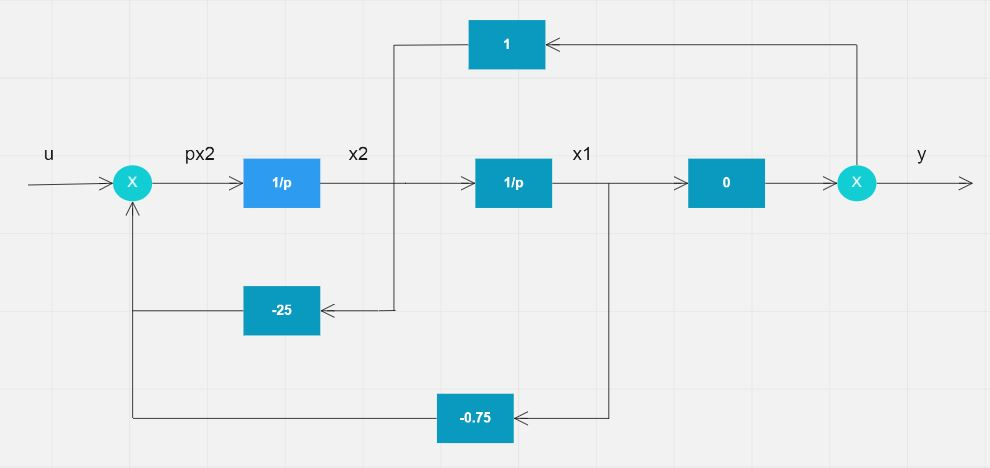
\includegraphics[scale = 0.73]{images/nfu.jpg}
	\caption{Система в форме управления}
	\label{image:1}
\end{figure}
\FloatBarrier

Её характеристики описываются матрицами:

\begin{equation*}
\text{$A=\begin{bmatrix} 0 & 1 \\ -0.75 & -2 \end{bmatrix}, 
	B=\begin{bmatrix} 0 \\ 1 \end{bmatrix}, 
	C=\begin{bmatrix} 0 & 1 \end{bmatrix}$}
\end{equation*}

При подключении управляющего устройства со структурой $U=-k_0x-k_1x'+gV$ получим, предполагая $x_2=x', x_1=x$:

\begin{figure}[h!]
	\centering
	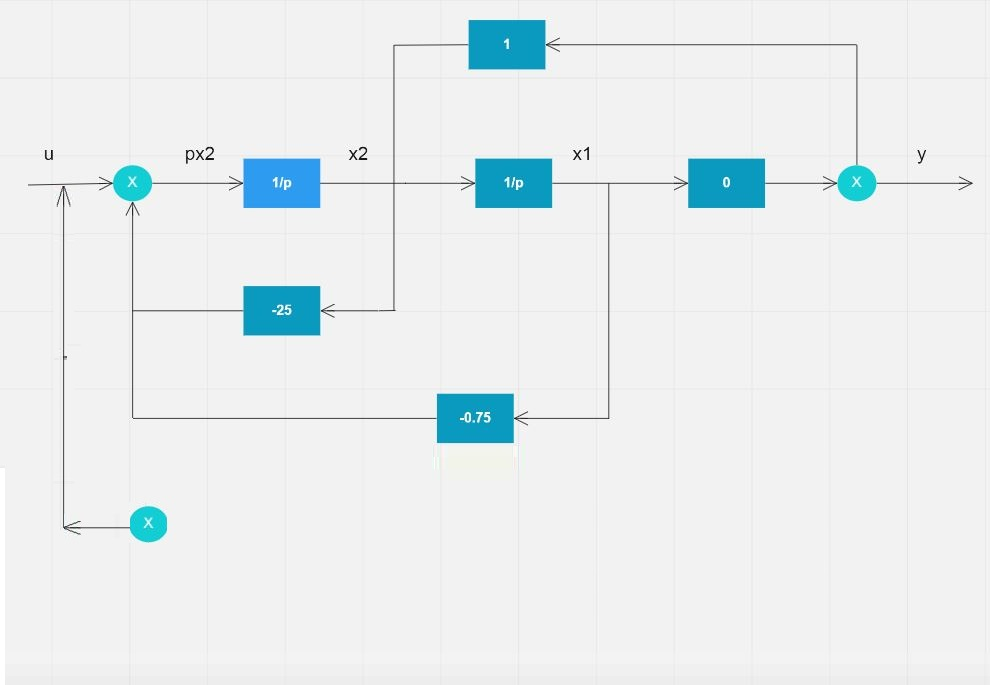
\includegraphics[scale = 0.73]{images/nfu2.jpg}
	\caption{Система с подключённым управляющим устройством}
	\label{image:2}
\end{figure}
\FloatBarrier

\chapter{Ход работы}

\section{Определение области устойчивости}

Для полученной системы определим, при каких значениях параметров УУ она будет устойчивой.
Сначала составим передаточную функцию. 

\begin{center}
	$W(p)=g*W_1(p)*W_2(p)=g*\frac{1/p}{1-1/p(-2-k_1+1/p(-0.75-k_0))}=g*\frac{p}{p^2+(k_1+2)p+(k_0+0.75)}$
\end{center}

Характеристический полином:
$p^2+(k_1+2)p+(k_0+0.75)$

Согласно критерию Гурвица для систем второго порядка, для устойчивости необходимо и достаточно, чтобы коэффициенты характеристического полинома были положительны, следовательно,

\begin{equation*}
\begin{cases}
\text{$k_0>-0.75$} \\
\text{$k_1>-2$}
\end{cases}
\end{equation*}

\section{Синтез оптимального УУ}

\subsection{Нахождение коэффициента обратной связи}

Синтезируем устройство, оптимальное по интегральному критерию:

\begin{center}
	$K=argmin[\int_{0}^{\inf}([x,x']^TQ[x,x']+U^TRUdt)]; Q=diag(a,b), R=1$.\\
	$K=R^{-1}(B^TS+N^T)$
\end{center}
	
Воспользуемся уравнением Рикатти:

\begin{center}
	$A^TS+SA-(SB+N)R^{-1}(B^TS+N^T)+Q=0$, 
\end{center}

где $S$-положительно определённая квадратная матрица. При этом $U=-KX$.

Вычислим коэффициенты обратной связи при $Q=E$:

\begin{center}
	$\begin{bmatrix} 0 & -0.75 \\ 1 & -2 \end{bmatrix}
	\begin{bmatrix} a & b \\ c & d \end{bmatrix}+
	\begin{bmatrix} a & b \\ c & d \end{bmatrix}
	\begin{bmatrix} 0 & 1 \\ -0.75 & -2 \end{bmatrix}-
	(\begin{bmatrix} a & b \\ c & d \end{bmatrix}
	\begin{bmatrix} 0 \\ 1 \end{bmatrix})
	(\begin{bmatrix} 0 & 1 \end{bmatrix}
	\begin{bmatrix} a & b \\ c & d \end{bmatrix})+
	\begin{bmatrix} 1 & 0 \\ 0 & 1 \end{bmatrix}=0$\\
	$\begin{bmatrix} -0.75c & -0.75d \\ a-2c & b-2d \end{bmatrix}+
	\begin{bmatrix} -0.75b & a-2b \\ -0.75d & c-2d \end{bmatrix}-
	(\begin{bmatrix} b \\ d \end{bmatrix}
	\begin{bmatrix} c & d \end{bmatrix})+
	\begin{bmatrix} 1 & 0 \\ 0 & 1 \end{bmatrix}=0$\\
	$\begin{bmatrix} -0.75c-50.7b & a-2b-0.75d \\ a-2c-0.75d & b+c-4d \end{bmatrix}-
	\begin{bmatrix} bc & bd \\ cd & d^2 \end{bmatrix}+
	\begin{bmatrix} 1 & 0 \\ 0 & 1 \end{bmatrix}=0$
\end{center}

\begin{center}
	$\begin{bmatrix} 1-bc-0.75c-0.75b & a-2b-bd-0.75d \\ a-2c-cd-0.75d & b+c+4d-d^2+1 \end{bmatrix}=0$
\end{center}

\begin{center}
	$a-2b-bd-0.75d=a-2c-cd-0.75d \Longrightarrow b(2-d)=c(2-d) \Longrightarrow b=c$\\
	$1-bc-0.75c-0.75b=0 \Longrightarrow -b^2-10b+1=0 \Longrightarrow b_{1,2}=\begin{bmatrix} -10.1, & 0.1 \end{bmatrix}$.
\end{center}

Известно, что $S$-положительно определённая матрица, поэтому $b=c=0.1$.

\begin{center}
	$-d^2-4d+1.2=0 \Longrightarrow d_{1,2}=\begin{bmatrix} 0.449, & -0.28 \end{bmatrix} \Longrightarrow d=0.449$.\\
	$a=bd+0.75d+2b=1.56$.
\end{center}

Таким образом, $S=\begin{bmatrix} 1.56 & 0.5 \\ 0.5 & 0.449 \end{bmatrix}, K=B^TS=\begin{bmatrix} 0.5 \\ 0.449 \end{bmatrix}$.

Данное решение удовлетворяет рассчитанным ранее критериям устойчивости.

\subsection{Нахождение коэффициента масштабирования}

Чтобы вычислить коэффициент g, масштабирующий входной сигнал, воспользуемся тем, что в установившемся режиме выход системы будет определяться как $y=gV_0*\frac{M}{M+1}$. Тогда при $g=\frac{M+1}{M}, y=V_0$, чего и требуется достичь.

Передаточная функция замкнутой системы: $W_3(p)=\frac{B(p)}{B(p)+C(p)}=\frac{p}{p^2+(k_1+2)p+(k_0+0.75)}$.

Тогда $W_p(p)=\frac{B(p)}{C(p)}=\frac{p}{p^2+(k_1+1)p+k_0+0.75}$.

Отсюда $M=W_p(0)=0$

Для ранее вычисленных значений $K=\begin{bmatrix} 0.5 \\ 0.449 \end{bmatrix}$ получим $M=0.8,g=2.25$.

\newpage

\section{Изучение влияния весовых коэффициентов на характерстики системы}

Изучим, как изменение одного из элементов весовой матрицы Q влияет на результирующие коэффициенты регулятора и на качество системы. Для этого будем фиксировать один из элементов, изменять другой и решать уравнение Риккати для данных значений.

Будем изменять один из параметров в пределах от 1 до 50 с шагом 5, а другой - фиксировать на значении 1.

\subsection{Изучение влияния весовых коэффициентов на параметры регулятора}

Получим следующие зависимости параметров регулятора от коэффициентов:

\begin{figure}[h!]
	\centering
	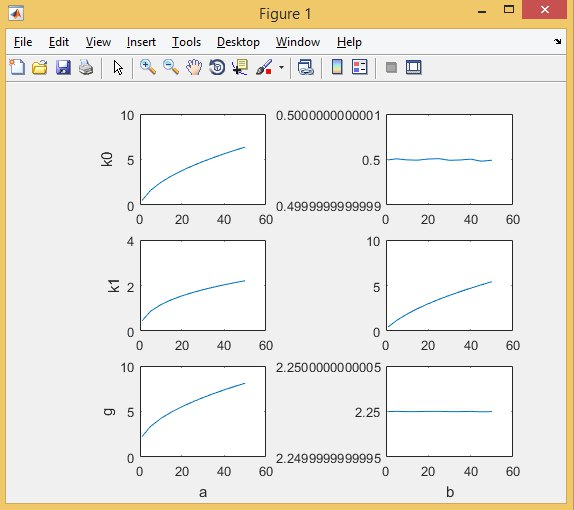
\includegraphics[scale = 0.55]{images/regq.png}
	\caption{Зависимость коэффициентов регулятора от параметров a, b}
	\label{image:3}
\end{figure}
\FloatBarrier

Данные зависимости объясняются следующим образом. Результирующие значения коэффициентов $K$ равны элементам $b$ и $d$ матрицы $S$. Значение $b$ определяется решением квадратного уравнения, свободный член которого линейно зависит от коэффициента $a$ матрицы $Q$, поэтому эти зависимости близки к линейным на рассмотренном промежутке. 

\subsection{Изучение влияния весовых коэффициентов на качество системы}

Аналогично изучим влияние весовых коэффициентов на показатели качества. Будем оценивать его по корневым критериям - среднему геометрическому корней характеристического полинома и степени устойчивости (минимальный модуль вещественной части корней). Кроме того, на первом графике в каждой группе указано значение максимальной из вещественных частей корней - это позволит отсечь случаи, когда система неустойчива.

\begin{figure}[h!]
	\centering
	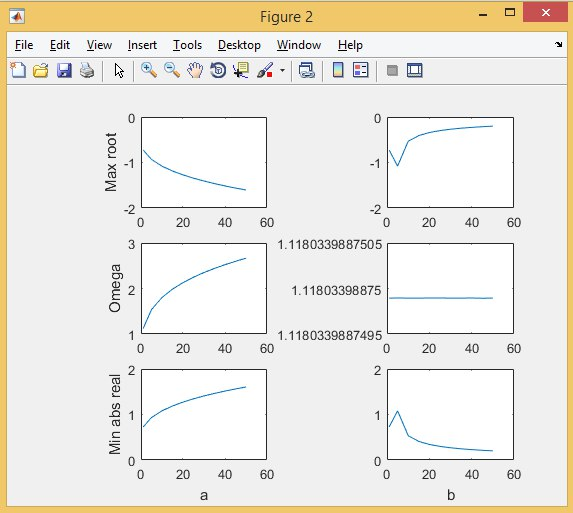
\includegraphics[scale = 0.55]{images/regs.png}
	\caption{Зависимость показателей качества от параметров a,b}
	\label{image:4}
\end{figure}
\FloatBarrier

Как видим, первая группа состоит из линейных зависимостей. Это объясняется тем, что сумма значений корней равна свободному члену характеристического полинома, который, в свою очередь, равен $k_0+5$, а зависимость $k_0$ от коэффициента $a$ близка к линейной при постоянном коэффициенте $b$. Среднегеометрическое значение корней практически не зависит от значения $b$. Как видно, система устойчива при рассмотренных значениях параметров. В общем и целом можно сказать, что увеличение весовых коэффициентов повышает качество системы. 

\section{Моделирование работы системы}

Смоделируем систему с поолученными оптимальными параметрами.

\begin{figure}[h!]
	\centering
	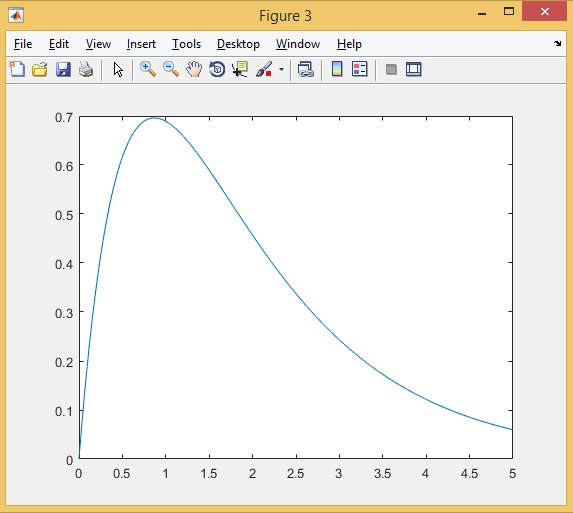
\includegraphics[scale = 0.73]{images/mod.png}
	\caption{Отклик системы при оптимальных значениях коэффициентов}
	\label{image:5}
\end{figure}
\FloatBarrier

\chapter{Вывод}

В ходе работы был изучен интегральный метод синтеза регулятора линейной системы.

При условии полной наблюдаемости системы регулятор может быть реализован через обратную связь от переменных пространства состояния. Результирующая система может быть путём структурных преобразований представлена в виде системы с обратной связью, что позволяет применить для неё весь математический аппарат, рассмотренный в предыдущих работах.

Для устойчивости системы необходимо соблюдение критериев устойчивости, в данном случае - $k_1>-2$ (искомые коэффициенты обратной связи рассматриваются как положительные).

Для линейных стационарных систем оптимальное решение может быть найдено путём решения матричного уравнения Риккати. Оно связывает матрицы системы и
оптимальные коэффициенты для управления вида $U=-KX$. В качестве показателя
оптимальности используется интегральный критерий.

Решение, оптимальное с точки зрения интегрального критерия, может привести к неустойчивости системы, поэтому результат всегда требует проверки.

Весовые коэффициенты матрицы Q оказывают влияние на получаемое решение.

Зависимости коэффициентов регулятора в большинстве случаев - линейные, как и зависимости  показателей качества. С ростом коэффициентов растёт качество решения.

\end{document}